\chapter{Lec 10 - Intro to Classification \& Model Selection}

\maketitle

\section{The Classification Setting}
Suppose that we seek to estimate $f$ on the basis of training observations $\{(x_1, y_1), ..., (x_n, y_n)\}$, where now $y_1,...,y_n$ are qualitative. The most common approach for quantifying the accuracy of our estimate $\hat{f}$ is the training error rate, the proportion of mistakes that are made if we apply our estimate $\hat{f}$ to the training observations:
\begin{equation}
    \frac{1}{n} \sum_{i=1}^n I(y_i \neq \hat{y}_i)
    \label{accuracy}
\end{equation}
Here $\hat{y}_i$ is the predicted class label for the $i$-th observation using $\hat{f}$. And $I(y_i \neq \hat{y}_i)$ is an indicator variable that equals 1 if $y_i \neq \hat{y}_i$ and zero if $y_i = \hat{y}_i$. Hence Equation \ref{accuracy} computes the fraction of incorrect classifications.\\\\
As in the regression setting, we are most interested in the error rates that result from applying our classifier to test observations that were not used in training. The \textit{test error} rate associated with a set of test observations of the form $(x_0, y_0)$ is given by
\begin{equation}
    Ave(I(y_0 \neq \hat{y}_0))
    \label{test-accuracy}
\end{equation}
A good classifier is one for which the test error \ref{test-accuracy} is smallest. It is possible to show that the test error rate given in \ref{test-accuracy} is minimized, on average, by a very simple classifier that assigns each observation to the most likely class, given its predictor values.  In other words, we should simply assign a test observation with predictor vector $x_0$ to the class $j$ for which
\begin{equation}
    P(Y=j | X=x_0)
    \label{cond prob}
\end{equation}
is largest. Note that \ref{cond prob} is a conditional probability: it is the probability that $Y = j$, given the observed predictor vector $x_0$. This very simple classifier is called the \textbf{Bayes classifier}. The Bayes classifier produces the lowest possible test error rate, called the \textit{Bayes error rate}.
\paragraph{K-Nearest Neighbors:} 
In theory we would always like to predict qualitative responses using the Bayes classifier. But for real data, we do not know the conditional distribution of $Y$ given $X$, and so computing the Bayes classifier is impossible. Therefore, the Bayes classifier serves as an unattainable gold standard against which to compare other methods. Many approaches attempt to estimate the conditional distribution of $Y$ given $X$, and then classify a given observation to the class with highest estimated probability.\\\\
One such method is the K-nearest neighbors (KNN) classifier. Given a positive integer $K$ and a test observation $x_0$, the KNN classifier first identifies the $K$ points in the training data that are closest to $x_0$, represented by $\mathcal{N}_0$. It then estimates the conditional probability for class $j$ as the fraction of points in $\mathcal{N}_0$ whose response values equal $j$:
\begin{equation}
    P(Y = j | X = x_0) = \frac{1}{K} \sum_{i \in \mathcal{N}_0} I(y_i = j)
\end{equation}
Finally, KNN applies Bayes rule and classifies the test observation $x_0$ to the class with the largest probability.
\begin{center}
    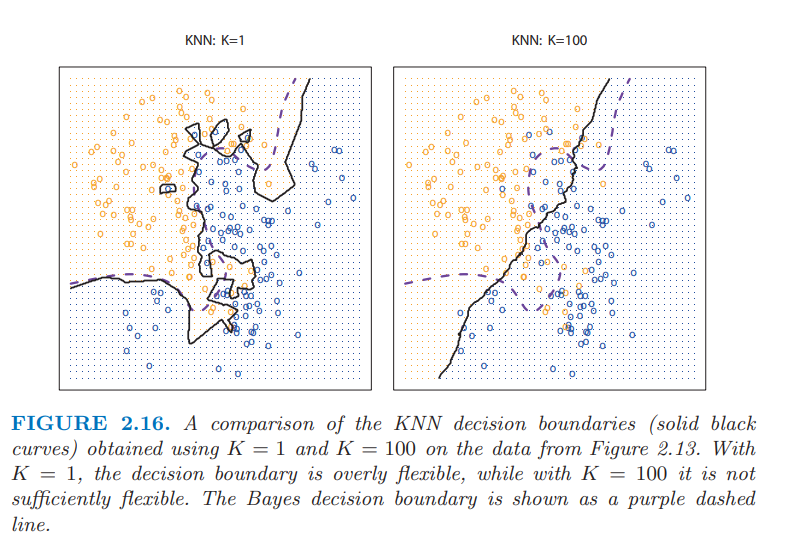
\includegraphics[scale=0.8]{images/knn-classification.png}
\end{center}
The choice of $K$ has a drastic effect on the KNN classifier obtained. When $K = 1$, the decision boundary is overly flexible and finds patterns in the data that don’t correspond to the Bayes decision boundary. This corresponds to a classifier that has low bias but very high variance. As $K$ grows, the method becomes less flexible and produces a decision boundary that is close to linear. This corresponds to a low-variance but high-bias classifier.
\begin{center}
    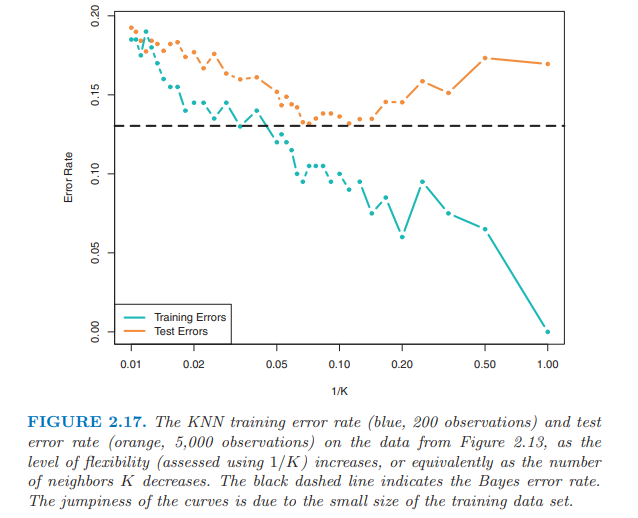
\includegraphics[scale=0.7]{images/knn-training-val error.png}
\end{center}
In Figure above, we have plotted the KNN test and training errors as a function of $1/K$. As $1/K$ increases, the method becomes more flexible. As in the regression setting, the training error rate consistently declines as the flexibility increases. However, the test error exhibits a characteristic U-shape, declining at first (with a
minimum at approximately$ K = 10$) before increasing again when the
method becomes excessively flexible and overfits.

\section{Cross-Validation}
In the absence of a very large designated test set that can be used to
directly estimate the test error rate, a number of techniques can be used to estimate this quantity using the available training data. Here we consider a class of methods that estimate the test error rate by holding out a subset of the training observations from the fitting process, and then applying the statistical learning method to those held out observations.

\subsection{The Validation Set Approach}
Suppose that we would like to estimate the test error associated with fitting a particular statistical learning method on a set of observations. The \textbf{validation set} approach is a very simple strategy for this task.  It involves randomly dividing the available set of observations into two parts, a training set and a \textit{validation set} or \textit{hold-out set}. The model is fit on the training set, and the fitted model is used to predict the responses for the observations in the validation set. The resulting validation set error rate—typically assessed using MSE in the case of a quantitative response—provides an estimate of the test error rate.
\begin{center}
    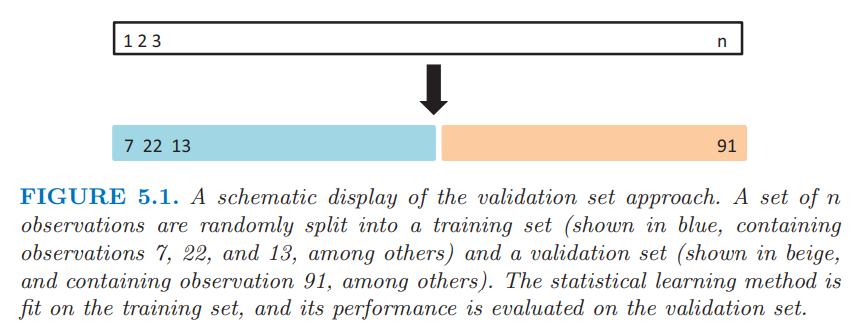
\includegraphics[scale=0.8]{images/cv.png}
\end{center}
The validation set approach is conceptually simple and is easy to implement. But it has two potential drawbacks:
\begin{enumerate}
    \item The validation estimate of the test error rate can be highly variable, depending on precisely which observations are included in the training set and which observations are included in the validation set.

    \item  In the validation approach, only a subset of the observations—those that are included in the training set rather than in the validation set—are used to fit the model. Since statistical methods tend to perform worse when trained on fewer observations, this suggests that the validation set error rate may tend to overestimate the test error rate for the model fit on the entire data set.

\end{enumerate}

\begin{center}
    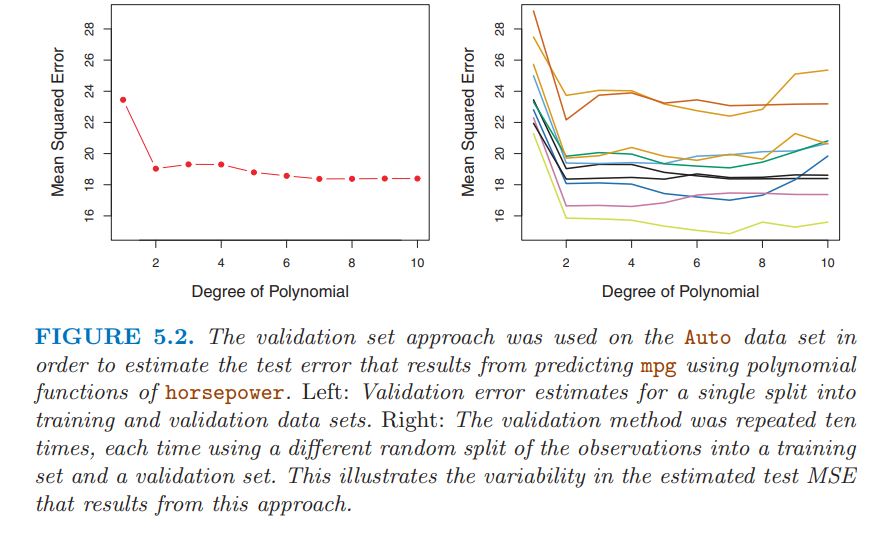
\includegraphics[scale=0.7]{images/cv2.png}
\end{center}
In the coming subsections, we will present \textit{cross-validation}, a refinement of the validation set approach that addresses these two issues.

\subsection{\textit{k}-Fold Cross-Validation}
This approach involves randomly dividing the set of observations into $k$ groups, or folds, of approximately equal size. The first fold is treated as a validation set, and the model is fit on the remaining $k - 1$ folds. The mean squared error, $MSE_1$, is then computed on the observations in the held-out fold. This procedure is repeated $k$ times; each time, a different group of observations is treated as a validation set. This process results in $k$ estimates of the test error, $MSE_1, MSE_2,..., MSE_k$. The $k$-fold CV estimate is computed by averaging these values
\begin{equation}
    CV_{(k)} = \frac{1}{k} \sum_{i=1}^k MSE_i
\end{equation}

\begin{center}
    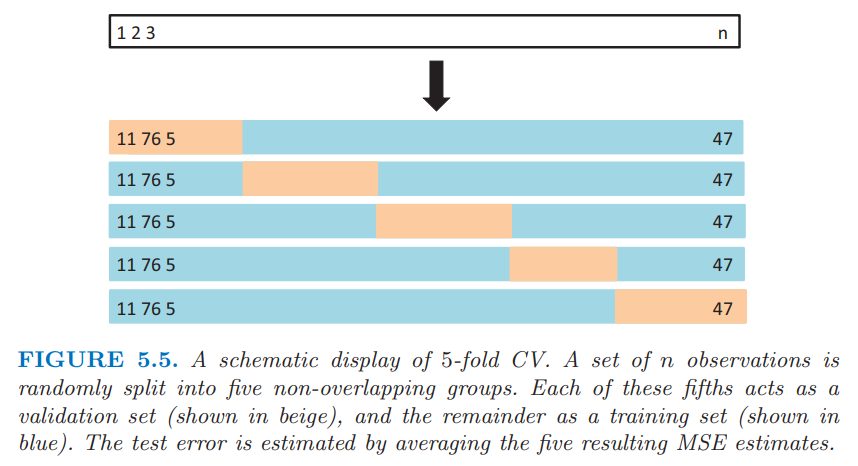
\includegraphics[scale=0.7]{images/k-fold-cv.png}
\end{center}
If we set $k=n$, we'll have $n$ folds or \textit{leave one out cross validation} (LOOCV).  In practice, one typically performs $k$-fold CV using $k = 5$ or $k = 10$. What is the advantage of using $k = 5$ or $k = 10$ rather than $k = n$? The most obvious advantage is computational. LOOCV requires fitting the statistical learning method $n$ times. This has the potential to be computationally expensive.  Putting computational issues aside, a less obvious but potentially more important advantage of $k$-fold CV is that it often gives more accurate estimates of the test error rate than does LOOCV. This has to do with a bias-variance trade-off.\\\\
Previously, we mentioned that the validation set approach can
lead to overestimates of the test error rate, since in this approach the training set used to fit the statistical learning method contains only half the observations of the entire data set. Using this logic, it is not hard to see that LOOCV will give approximately unbiased estimates of the test error, since each training set contains $n - 1$ observations, which is almost as many as the number of observations in the full data set.\\\\
However, we know that bias is not the only source for concern in an estimating procedure; we must also consider the procedure’s variance. It turns out that LOOCV has higher variance than does $k$-fold CV with $k<n$. Why is this the case? When we perform LOOCV, we are in effect averaging the outputs of $n$ fitted models, each of which is trained on an almost identical set of observations; therefore, these outputs are highly (positively) correlated with each other. Since the mean of many highly correlated quantities has higher variance than does the mean of many quantities that are not as highly correlated, the test error estimate resulting from LOOCV tends to have higher variance than does the test error estimate resulting from $k$-fold CV.\\\\
To summarize, there is a bias-variance trade-off associated with the
choice of $k$ in $k$-fold cross-validation. Typically, given these considerations, one performs $k$-fold cross-validation using $k = 5$ or $k = 10$, as these values have been shown empirically to yield test error rate estimates that suffer neither from excessively high bias nor from very high variance.\\\\
When we perform cross-validation, our goal might be to determine how
well a given statistical learning procedure can be expected to perform on independent data; in this case, the actual estimate of the test MSE is of interest. But at other times we are interested only in the location of the minimum point in the estimated test MSE curve. This is because we might be performing cross-validation on a number of statistical learning methods, or on a single method using different levels of flexibility, in order to identify the method that results in the lowest test error.
\begin{center}
    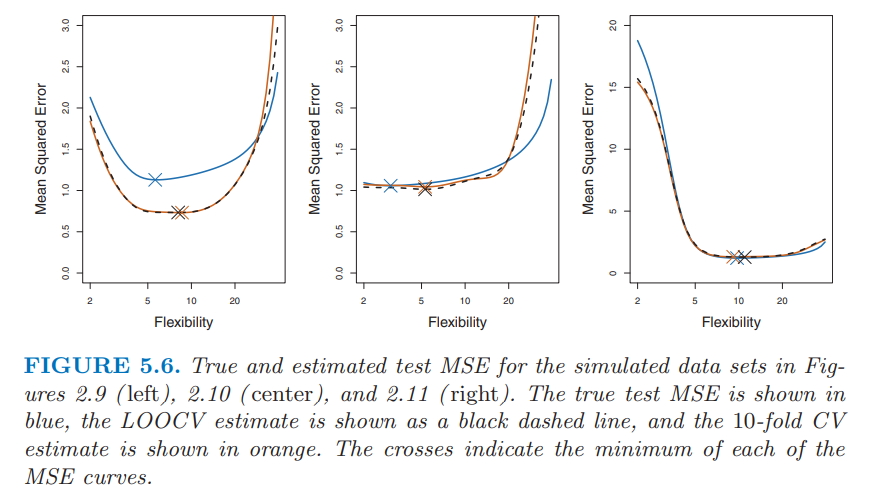
\includegraphics[scale=0.7]{images/k-fold-cv2.png}
\end{center}

\subsubsection{Data Leakage}
One common mistake which arises when performing $k$-fold cross validation is the so called \textit{data leakage} problem. In the context of $k$-fold cross validation, a common mistake is to perform data preparation on the entire dataset \textit{before} performing the cross validation procedure. Although this is a common approach, it is dangerously incorrect in most cases. 
\\\\
The problem with applying data preparation techniques before splitting data for model evaluation is that it can lead to data leakage and, in turn, will likely result in an incorrect estimate of a model’s performance.\\\\
Data leakage refers to a problem where information about the holdout dataset, such as a test or validation dataset, is made available to the model in the training dataset. This leakage is often small and subtle but can have a marked effect on performance.\\\\
The solution is straightforward: data preparation must be fit only on the training set inside the $k$-fold cross validation loop. That is, any coefficients or models prepared for the data preparation process must only use rows of data in the training dataset. Once fit, the data preparation algorithms or models can then be applied to the training set, and to the test set. This might include data transforms, but also other techniques such feature selection, dimensionality reduction, feature engineering and more. 
